%%%%%%%%%%%%%%%%%%%%%%%%%%%%%%%%%%%%%%%%%%%%%%%%%%%%%%%%%%%%%%%%%%%%%%%%%%%%%%%%
%2345678901234567890123456789012345678901234567890123456789012345678901234567890
%        1         2         3         4         5         6         7         8
%% PP_Report.tex
%% V2.1
%% 2017/05/07
%% by Rui Santos Cruz
%% This is a skeleton file using PPIEEEtran.cls
%% (requires PPIEEEtran.cls) 
% !TEX root = ./main.tex
%%%%%%%%%%%%%%%%%%%%%%%%%%%%%%%%%%%%%%%%%%%%%%%%%%%%%%%%%%%%%%%%%%%%%%%%%%%%%%%%
\documentclass[a4paper,12pt,journal,twoside,compsoc]{PPIEEEtran}

% In the ReportType command chose "act" for Activity Report or "learn" for Learnings Report
\newcommand*{\ReportType}{learn}
% -----------------------------------------------------------------------------
% The Preamble document contains all the necessary Packages for typesetting
% Modify it to suit your needs
% -----------------------------------------------------------------------------
%%%%%%%%%%%%%%%%%%%%%%%%%%%%%%%%%%%%%%%%%%%%%%%%%%%%%%%%%%%%%%%%%%%%%%%%%%%%%%%%
%2345678901234567890123456789012345678901234567890123456789012345678901234567890
%        1         2         3         4         5         6         7         8
% Required Packages and commands
% --> Please Choose the MAIN LANGUAGE for the document in package BABEL (below)
% --> Please Choose the TYPE OF REPORT for the document in \ReportType (below)
% !TEX root = ./main.tex
% PP_Report_Preamble.tex
% V2.1
% 2017/05/07
% by Rui Santos Cruz
%%%%%%%%%%%%%%%%%%%%%%%%%%%%%%%%%%%%%%%%%%%%%%%%%%%%%%%%%%%%%%%%%%%%%%%%%%%%%%%%
%
% *** INPUT LANGUAGE PACKAGES ***
% Choose the main language in package Babel
\usepackage[english,main=portuguese]{babel}
\usepackage[utf8]{inputenc}
\usepackage{iflang}

% *** ACRONYM PACKAGES ***
% Put definition of Acronyms at the end of the document
\usepackage[printonlyused,nolist]{acronym}

% *** CITATION PACKAGES ***
\usepackage{cite}

% *** GRAPHICS RELATED PACKAGES ***
\usepackage[pdftex]{graphicx}
\DeclareGraphicsExtensions{.pdf,.jpeg,.png}

% *** MATH PACKAGES ***
\usepackage[cmex10]{amsmath}

% *** SPECIALIZED LIST PACKAGES ***
\usepackage{algorithmic}

% *** ALIGNMENT PACKAGES ***
\usepackage{array}

% *** SUBFIGURE PACKAGES ***
\usepackage[caption=false,font=normalsize,labelfont=sf,textfont=sf]{subfig}

% *** FLOAT PACKAGES ***
\usepackage{fixltx2e}

% *** PDF, URL AND HYPERLINK PACKAGES ***
\usepackage{url}

% *** BACKGROUND Material ***
\usepackage{eso-pic}
\usepackage[
  contents={},
  opacity=1,
  scale=1,
  color=blue!90
  ]{background}
  
% *** CONDITIONALS ***
\usepackage{ifthen}

% Clever Referencing
% Note: portuguese is supported through "brazilian" option
\usepackage[\IfLanguageName{english}{english}{brazilian}]{cleveref}

%%%%%%%%%%%%%%%%%%%%%%%%%%%%%%%%%%%%%%%%%%%%%%%%%%%%%%%%%%%%%%%%%%%%%%%%%%%%%%%%
% PLEASE DO NOT CHANGE THIS SECTION
% Printing the Scoring Table
\AddToShipoutPicture*{\BackgroundPic}
%%%%%%%%%%%%%%%%%%%%%%%%%%%%%%%%%%%%%%%%%%%%%%%%%%%%%%%%%%%%%%%%%%%%%%%%%%%%%%%%
% PLEASE DO NOT CHANGE THIS SECTION
% Print Vertical Identifications on even and odd pages
\AddEverypageHook{%
  \ifthenelse{\isodd{\value{page}}}%
  {\backgroundsetup{
    angle=90,
    position={-0.1\textwidth,-1.055\textheight},
    contents={\tiny{PP-2017 V2.1}}
    }% Odd Pages
  }%
  {\backgroundsetup{
    angle=90,
    position={0.97\textwidth,-1.05\textheight},%
    contents={\ifthenelse{\equal{\ReportType}{act}}{%
              \tiny{\tlangRepActivity}}{\tiny{\tlangRepLearning}}}
    }% Even Pages
  }%
  \BgMaterial}
  %%%%%%%%%%%%%%%%%%%%%%%%%%%%%%%%%%%%%%%%%%%%%%%%%%%%%%%%%%%%%%%%%%%%%%%%%%%%%%%%
% correct bad hyphenation here
\hyphenation{op-tical net-works semi-conduc-tor}
%%%%%%%%%%%%%%%%%%%%%%%%%%%%%%%%%%%%%%%%%%%%%%%%%%%%%%%%%%%%%%%%%%%%%%%%%%%%%%%%
%2345678901234567890123456789012345678901234567890123456789012345678901234567890
%        1         2         3         4         5         6         7         8
\begin{document}

%%%%%%%%%%%%%%%%%%%%%%%%%%%%%%%%%%%%%%%%%%%%%%%%%%%%%%%%%%%%%%%%%%%%%%%%%%%%%%%%
%2345678901234567890123456789012345678901234567890123456789012345678901234567890
%        1         2         3         4         5         6         7         8
%% PP_Report_Cover.tex
%% V2.1
%% 2017/05/07
%% by Rui Santos Cruz
% !TEX root = ./main.tex
%%%%%%%%%%%%%%%%%%%%%%%%%%%%%%%%%%%%%%%%%%%%%%%%%%%%%%%%%%%%%%%%%%%%%%%%%%%%%%%%
% paper title
% can use linebreaks \\ within to get better formatting as desired
% Do not put math or special symbols in the title.
\title{Deteção de eventos em discursos políticos}

%%%%%%%%%%%%%%%%%%%%%%%%%%%%%%%%%%%%%%%%%%%%%%%%%%%%%%%%%%%%%%%%%%%%%%%%%%%%%%%%
% Author names
%
% note positions of commas and nonbreaking spaces ( ~ ) LaTeX will not break
% a structure at a ~ so this keeps an author's name from being broken across
% two lines.
% use \thanks{} to gain access to the first footnote area
% a separate \thanks must be used for each paragraph.
%
%\IEEEcompsocitemizethanks is a special \thanks that produces the bulleted
% lists for "first footnote" author affiliations. 
% Use \IEEEcompsocthanksitem which works much like \item
% for each affiliation group.
\author{Gonçalo~Fialho~Pires,
        Pedro~Miguel~Duarte% <-this % stops a space
% Change the Course Name 
% note: need leading \protect in front of \\ to get a newline within \thanks as
% \\ is fragile and will error, could use \hfil\break instead.
\IEEEcompsocitemizethanks{
\IEEEcompsocthanksitem Gonçalo~Fialho~Pires, nr. 79112,\protect\\ 
E-mail: goncalo.f.pires@tecnico.ulisboa.pt,
\IEEEcompsocthanksitem Pedro~Duarte, nr. 78328,\protect\\
E-mail: pedro.m.duarte@tecnico.ulisboa.pt,\protect\\
Instituto Superior Técnico, Universidade de Lisboa.\protect\\}% <-this % stops an unwanted space}% <-this % stops an unwanted space
\thanks{Manuscrito recebido a 1 de Junho de 2018.}
}
%%%%%%%%%%%%%%%%%%%%%%%%%%%%%%%%%%%%%%%%%%%%%%%%%%%%%%%%%%%%%%%%%%%%%%%%%%%%%%%%
% The paper headers
\markboth{Deteção de eventos em discursos políticos}%
% for a single student
%{Surname}% : for a single student 
% for a Group Report 
{Duarte \MakeLowercase{\textit{et al.}}}% : for a Group Report 
%
% The only time the second header will appear is for the odd numbered pages
% after the title page when using the twoside option.

%%%%%%%%%%%%%%%%%%%%%%%%%%%%%%%%%%%%%%%%%%%%%%%%%%%%%%%%%%%%%%%%%%%%%%%%%%%%%%%%
% Prints in Subtitle the type of Report
% PLEASE DO NOT CHANGE THIS SECTION
\IEEEspecialpapernotice{%
\ifthenelse{\equal{\ReportType}{act}}{%
\tlangRepActivity}{\tlangRepLearning}
}
%%%%%%%%%%%%%%%%%%%%%%%%%%%%%%%%%%%%%%%%%%%%%%%%%%%%%%%%%%%%%%%%%%%%%%%%%%%%%%%%
%%%%%%%%%%%%%%%%%%%%%%%%%%%%%%%%%%%%%%%%%%%%%%%%%%%%%%%%%%%%%%%%%%%%%%%%%%%%%%%%
% The paper Abstract and Keywords
\IEEEtitleabstractindextext{%

\begin{abstract}
This report will discuss what I learned during my activity when organizing the Global Game Jame edition of 2018, in the Taguspark campus. It shows just how important soft-skills are in any workplace environment and how it affected my growth as a student. It also includes an overall assessment of the activity and my learning process.
\end{abstract}
%
\begin{IEEEkeywords}
Soft-skills, Event Organization
\end{IEEEkeywords}}
%%%%%%%%%%%%%%%%%%%%%%%%%%%%%%%%%%%%%%%%%%%%%%%%%%%%%%%%%%%%%%%%%%%%%%%%%%%%%%%%

% make the title area
\maketitle

\IEEEdisplaynontitleabstractindextext
\IEEEpeerreviewmaketitle
%%%%%%%%%%%%%%%%%%%%%%%%%%%%%%%%%%%%%%%%%%%%%%%%%%%%%%%%%%%%%%%%%%%%%%%%%%%%%%%%
%%%%%%%%%%%%%%%%%%%%%%%%%%%%%%%%%%%%%%%%%%%%%%%%%%%%%%%%%%%%%%%%%%%%%%%%%%%%%%%%
\section{Introduction}
% The very first letter is a 2 line initial drop letter followed
% by the rest of the first word in caps (small caps for compsoc).
% 
% form to use if the first word consists of a single letter:
% \IEEEPARstart{A}{demo} file is ....
% 
% Here we have the typical use of a "E" for an initial drop letter
% and "STE" in caps to complete the first word.
\IEEEPARstart{S}{oft} skills are a very important part of anyone that has the objective of contributing positively to society. This is because, while they do not depend on acquired knowledge of some technical field of study, they are vital to better understanding the people one inevitably needs to communicate with on a daily basis when performing any kind of job, even if technical job. In \cite{workforce}, soft-skills are described as a combination of people skills, social skills, communication skills, character traits and attitudes that one must have in order to perform effectively in any environment and work well with others. They actively complement a person's hard-skills and are crucial to a balanced workforce, mainly because any environment is filled with people and people are the engine of society, i.e. they drive service jobs and technical jobs, and the better the communication and cooperation, the better the end product of any of these jobs.

In the scope of better understanding the importance of soft-skills, it is believed that the best way to do this is through experience. With this in mind, and in the scope of the Independent Studies 1 course, it was proposed to all students to choose any activity with the objective of improving their soft-skills and better understand why it is such a crucial part of one's set of available tools through their lives. To achieve this goal, I choose the institutional activity of "Organization of the IST participation at the Global Game Jam 2018", from the institution IST, Instituto Superior Técnico. The goal of this activity is to support the organization of IST behind the Global Game Jam that takes place in January 2018, on the days 26 to 28. This is a worldwide event where the participants must complete a game from scratch in the period of 48 hours. Because this is a worldwide event, many clusters are organized through the world and need to be synchronized to start the event at the same time. With this, IST are collaborating with the Faculdade de Belas Artes da Universidade de Lisboa in the organization of the event in Lisbon and so, in the 26-28 of January, students will gather in the facilities of IST - Taguspark to attend to this worldwide event. This activity is an initiative by the Games Lab (http://labjogos.tecnico.ulisboa.pt/) of IST and because this is a big-scale event, it a lot of additional manpower. 

In the rest of this report, I will describe what lead me to choose this activity, as well as what skills I believe were improved over the past weeks. Finally, because it is also important to be constructively critic about nearly everything in life, I will provide a critic overview of my progress as well as on the activity itself.

The organization of this document is as follows: \cref{motivation} describes the motivation behind my choice of activity; \cref{skills} discusses the skills that I improved when doing the activity; \cref{reflection} provides a critical self-evaluation of my performance in the activity as well as possible improvements. Finally, \cref{concl} concludes this report.

%%%%%%%%%%%%%%%%%%%%%%%%%%%%%%%%%%%%%%%%%%%%%%%%%%%%%%%%%%%%%%%%%%%%%%%%%%%%%%%%
\section{Motivation}
\label{motivation}

Because I grew up in the 90's, where video games had began to grow and became a huge success with of that decade, I have always been a huge fan of games and this also played a huge part in pursuing a career related to technologies, more specifically in Computer Science, as the curiosity of how games were made and how a bunch of lines of code resulted in something as intricate as a computer program led me to wanting to know more. 

Years later, I am given the opportunity to help organizing an event that focuses on team work, even with students of other universities, to build a game from nothing in 48 hours. No doubt the technical skills here are also a must-have, but it very difficult to see a team that has no communication skills reach a satisfactory final result. With this said, the fun of competing against other teams and the communication and cooperation aspect with one's own team made me participate in the Global Game Jam of 2017. Because I enjoyed the experience so much, I decided to participate as well in this year's edition and also help organizing the event, with the additional motivation of being a proposed institutional activity for the Independent Studies 1 course.

%%%%%%%%%%%%%%%%%%%%%%%%%%%%%%%%%%%%%%%%%%%%%%%%%%%%%%%%%%%%%%%%%%%%%%%%%%%%%%%%
%%%%%%%%%%%%%%%%%%%%%%%%%%%%%%%%%%%%%%%%%%%%%%%%%%%%%%%%%%%%%%%%%%%%%%%%%%%%%%%%
\section{Skills}
\label{skills}
This section will describe the skills that I learned up to this point in the scope of my activity, such as teamwork or time management ability, as is the objective of this report. Note that, because the actual event did not occur yet, I believe the following skills will be improved even further.

\subsection{Communication Ability}

Communication ability is the skill that allows a person to orally speak in public, write better reports (e.g. this one), present their ideas and to also better listen to other people. This is the most important skill according to the top 10 list of most important soft-skills in \cite{executive}. In spite of the many group projects I had to do in the past, I believe my communication ability still had a lot of room for improvement, and that is what happened: when having to discuss ideas with fellow students that are also a part of the organization of the Global Game Jam and when having to contact potential sponsors. 

\subsection{Teamwork}

Teamwork is the 9th ranked soft-skill in \cite{executive}, and it is a skill that focuses on the cooperation between member of a certain social or work circle and in the continuous support of its members among themselves. This skill was improved in the form of constant communication and help among the rest of the organizers, e.g. when someone had doubts about some aspect of the organization, the rest would try to give their opinion and help on the matter.

\subsection{Interpersonal Skills}

This skill is one that is inherent to most humans: the tendency to be warm and kind to one another, friendly and patient. At a glance, it might not even seem to be that important, however it is placed in 5th in the top social skills of \cite{executive}. Without this, work environments would be a cold and uncomfortable place, unsuited for any kind of work that vises to accomplish something beneficial to society. The work environment of the GGJ organization was very friendly and allowed for more open and comfortable discussions about the event.

\subsection{Decision Making Ability}

This ability is what helps people decide quickly and efficiently when confronted with a problem. It is crucial because without this most people would dabble infinitely on one difficult problem and never actually getting to solve it. In multiple occasions some of the decisions I made made me think back and actually consider if I made the right decision, but a wrong decision is better than no decision at all.

\subsection{Flexibility}

Flexibility is placed in the 3rd place of the list in \cite{executive}, and is the ability to adapt and accept new things, as well as a capacity to adjust to better work with the current situation, no matter how worse it is. I believe I had the opportunity to improve this ability in this activity, because originally I was in the logistics team, but after I was also put in the sponsors team and had to adapt my original work flow.

\subsection{Negotiation Ability}

Because I had to contact with potential sponsors, I believe my negotiation ability also improved a lot. This is because I had to make sure both parties were satisfied with my proposition. Negotiation ability is very important to make sure negotiations go smoothly for all involved, and are as efficient as possible. 

%%%%%%%%%%%%%%%%%%%%%%%%%%%%%%%%%%%%%%%%%%%%%%%%%%%%%%%%%%%%%%%%%%%%%%%%%%%%%%%%
%%%%%%%%%%%%%%%%%%%%%%%%%%%%%%%%%%%%%%%%%%%%%%%%%%%%%%%%%%%%%%%%%%%%%%%%%%%%%%%%

\section{Reflection}
\label{reflection}

In this section, a critic assessment of my performance and learning process will be made, as well as an overall evaluation of the activity and organization up to this point.

\subsection{Personal Performance}

I believe I did my best in any of the tasks that were proposed to me, such as the involvement in the sponsors team and when looking for things to buy for the event, in the logistics team. I also believe that, since the actual event did not occur yet, I still have some time to reflect on the activity thus far and use this knowledge to better serve the organization of this event in the Taguspark campus as part of the logistics team. There was a good amount of communication and teamwork from me and my colleagues and, overall, I feel satisfied with my performance.

\subsection{Activity Evaluation}

Since the actual event did not occur yet, I cannot evaluate how good it will go. However, since I have some knowledge of how things are supposed to go (since I attended the edition of the previous year) I believe I have the information necessary at my disposal to make sure it goes as smoothly as possible. 
On the actual activity up to this point: although my tasks were not that difficult, I still received a good amount of help from everyone, since it was my first time doing something of this sort, and I am pleased with the activity overall, as well as the rest of the organization of this event.

\section{\IfLanguageName{english}{Conclusion}{Conclusão}}
\label{concl}
Overall, I am very pleased on how things turned out, since a good amount of work is already done before the event even starts, and this shows just how much preparation is needed and how much teamwork and communication is necessary to make things go smoothly. It is good to note too that the skills I learned will prove to be very useful in the future, and the connections I made were also very important.
%%%%%%%%%%%%%%%%%%%%%%%%%%%%%%%%%%%%%%%%%%%%%%%%%%%%%%%%%%%%%%%%%%%%%%%%%%%%%%%%
%%%%%%%%%%%%%%%%%%%%%%%%%%%%%%%%%%%%%%%%%%%%%%%%%%%%%%%%%%%%%%%%%%%%%%%%%%%%%%%%
% use section* for acknowledgement
\ifCLASSOPTIONcompsoc
  % The Computer Society usually uses the plural form
  \section*{\IfLanguageName{english}{Acknowledgments}{Agradecimentos}} % Acknowledgments
\else
  % regular IEEE prefers the singular form
  \section*{Acknowledgment}
\fi

I would like to thank professor Carlos Martinho for allowing me to become a part of the organization of the \ac{GGJ} of the Taguspark, and my fellow colleagues for working with me.
%%%%%%%%%%%%%%%%%%%%%%%%%%%%%%%%%%%%%%%%%%%%%%%%%%%%%%%%%%%%%%%%%%%%%%%%%%%%%%%%

% references section
\bibliographystyle{IEEEtran}
%\bibliography{PP_Report_bib}
\bibliography{Mendeley}
%%%%%%%%%%%%%%%%%%%%%%%%%%%%%%%%%%%%%%%%%%%%%%%%%%%%%%%%%%%%%%%%%%%%%%%%%%%%%%%%
% biography section
% 

\begin{IEEEbiography}[{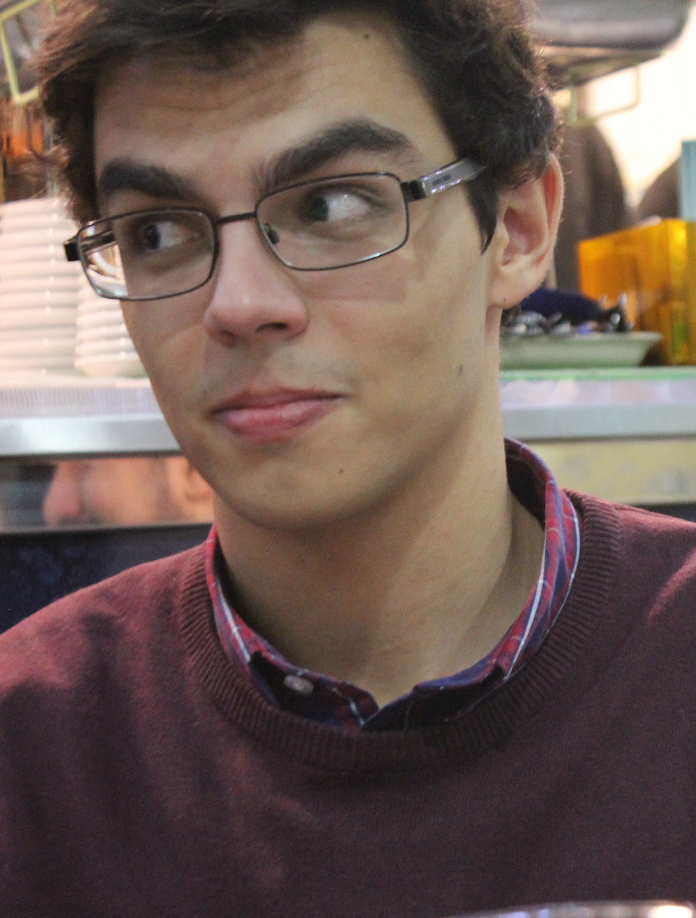
\includegraphics[width=1in,height=1.25in,clip,keepaspectratio]{me.png}}]{Pedro Miguel dos Santos Duarte}
I am currently pursuing my Master's Degree in Engineering studies at \ac{IST}, specializing in Intelligent Systems and Information Systems. I strive to make this world a better place for everybody living in it and I am always ready to take on a challenge.
\end{IEEEbiography}

%%%%%%%%%%%%%%%%%%%%%%%%%%%%%%%%%%%%%%%%%%%%%%%%%%%%%%%%%%%%%%%%%%%%%%%%%%%%%%%%

% *** DEFINITION OF ACRONYMS ***
	\acrodef{GGJ}{Global Game Jam}
	\acrodef{IST}{Instituto Superior Técnico}
	
% that's all folks
\end{document}